%!TEX option = -shell-escape
%!TEX builder = latexmk
%!TEX program = xelatex
\documentclass{beamer}
% ----- Loadings -----
\newif\ifcompile\compilefalse
\usetheme[menuwidth={0.7\paperwidth}]{erlangen}
\setbeamercovered{transparent=8}
\graphicspath{{./figures/}}
\usepackage{tipa}
\usepackage{xeCJK}
\usepackage{hologo}
\usepackage{multicol}
\usepackage{hyperref}
\usepackage{amsmath}
\usepackage{amssymb}
\usepackage{filecontents}
\usepackage{minted}

% ----- Font Set -----
\setCJKmainfont[AutoFakeSlant, BoldFont = FZHTK.TTF]{FZZDXK.TTF}
\setCJKmonofont[AutoFakeSlant, AutoFakeBold]{FZFSK.TTF}
% ----- New Commands -----
\newcommand{\ChinaTeX}{China\hologo{TeX}}
\renewcommand{\TeX}{\hologo{TeX}}
\renewcommand{\LaTeX}{\hologo{LaTeX}}
\renewcommand{\eTeX}{\hologo{eTeX}}
\newcommand{\pdfTeX}{\hologo{pdfTeX}}
\newcommand{\pdfLaTeX}{\hologo{pdfLaTeX}}
\newcommand{\XeTeX}{\hologo{XeTeX}}
\newcommand{\XeLaTeX}{\hologo{XeLaTeX}}
\newcommand{\LuaTeX}{\hologo{LuaTeX}}
\newcommand{\ConTeXt}{\hologo{ConTeXt}}
\newcommand{\BibTeX}{\hologo{BibTeX}}
\newcommand{\MiKTeX}{\hologo{MiKTeX}}
\newcommand{\TeXLive}{\TeX{} Live}
\newcommand{\pTeX}{p\TeX}
\newcommand{\upTeX}{up\TeX}
\newcommand{\eupTeX}{\ensuremath{\varepsilon}-up\TeX}
\newcommand{\OMEGA}{Omega}
\newcommand{\pTeXng}{\pTeX{}-ng}
\newcommand{\CTeX}{\ensuremath{\mathbb{C}}\TeX}
\newcommand{\MacTeX}{Mac\TeX}
\newcommand{\LaorTeX}{(\hologo{La})\TeX}
\newcommand{\PlainTeX}{Plain \TeX}
\makeatletter
\newcommand{\mheader}[1]{\gdef\@cm@header{#1}}
\makeatother
\newcommand{\pkg}[1]{\textsf{#1}}
\newcommand{\file}{\textsf}
\setbeamertemplate{background}{}
\setlength{\parskip}{0.5ex}
\usemintedstyle{perldoc}

% ----- Title Set -----
\title[宏包简介与数学建模美赛模板]{\ChinaTeX{} 在线培训课程}
\subtitle{宏包简介与数学建模美赛模板}
\author{Liam Huang}
\date{\today}
\institute{Shandong University\\[-0.2em]{\small School of Mathematics}}
\mheader{\ChinaTeX{} 在线培训课程}

\begin{document}

\begin{frame}[plain]
  \titlepage
\end{frame}

\begin{frame}{目录}
\tableofcontents
\end{frame}

\section{\TeX{} 发行版的目录结构}

\begin{frame}
  \sectionframe{\TeX{} 发行版的目录结构}
\end{frame}

\begin{frame}{\LaTeX{} 中常见的文件类型}
  \begin{itemize}
    \item \file{.tex} - 文章源代码
    \item \file{.cls} - 文档类(class)
    \item \file{.sty} - 宏包(style)\pause
    \item \file{.bib} - \BibTeX{} 数据库文件
    \item \file{.bst} - \BibTeX{} 样式文件(bibliography style)\pause
    \item \file{.ins} - 宏包安装文件(install)
    \item \file{.dtx} - 文档化的宏包源代码(documented tex source)\pause
    \item \file{.map}, \file{.tfm} ...
  \end{itemize}
\end{frame}

\begin{frame}{TDS (\TeX{} Directory Structure)}
  \TeXLive{} 中有超过 14 万个文件,\LaTeX{} 是怎么找到所需的文件的呢?
  \begin{itemize}
    \item 按照 TDS 的规则,分门别类,放在指定位置\pause
    \item TDS 的根目录叫做 TEXMF (\TeX{} and \hologo{METAFONT})
      \begin{itemize}
        \item TEXMF 可以有多个,相互独立
        \item 优先级 \\
          TEXMFLOCAL (texmf-local) $ > $ TEXMFDIST (texmf-dist)
      \end{itemize}\pause
    \item ls-R 数据库
      \begin{itemize}
        \item mktexlsr
        \item texhash
      \end{itemize}\pause
    \item kpsewhich 命令和 texdoc 命令
  \end{itemize}
\end{frame}

\section{宏包和文档类的安装}

\begin{frame}
  \sectionframe{宏包和文档类的安装}
\end{frame}


\begin{frame}{使用宏包管理器安装}
  \begin{itemize}
    \item \MiKTeX{} Package Manager (命令行执行 mpm)\pause
    \item \TeXLive Manager (命令行执行 tlmgr)
    \begin{itemize}
      \item tlmgr info \emph{package}\pause
      \item tlmgr option repository
      \item tlmgr option repository \url{http://mirror.ctan.org/systems/texlive/tlnet}\pause
      \item tlmgr update -{}-self
      \item tlmgr update -{}-all
      \item tlmgr update \emph{package}\pause
      \item tlmgr -{}-gui
    \end{itemize}
  \end{itemize}
\end{frame}

\begin{frame}{手工安装}
  \begin{itemize}
    \item TDS 安装包\pause
    \item 处理 \file{.ins} 文件\pause
    \item 处理 \file{.dtx} 文件\footnote{参考:\url{http://www.zhihu.com/question/27693438/answer/37669407}、\\\qquad\url{http://liam0205.me/2015/01/23/literate-programming-in-latex/}}
  \end{itemize}
\end{frame}

\section{美赛模板简介}

\begin{frame}
  \sectionframe{美赛模板简介}
\end{frame}

\begin{frame}{标题页控制 - Team Control Number}
  \begin{itemize}
    \item 每一个参赛队伍都有一个唯一的控制号码(Team Control Number)
    \item 控制页(Control Sheet)和正文页眉\pause
    \item 参数 tcn 用于设定控制号码\\
      tcn = 12345
  \end{itemize}
\end{frame}

\begin{frame}{标题页控制 - Control Sheet}
  \begin{itemize}
    \item sheet 选项为真时,显示控制页;反之不显示。\pause
    \item titleinsheet 选项为真时,在控制页显示文章标题;反之不显示。
    \item keywordsinsheet 选项为真时,在控制页显示关键字;反之不显示。
  \end{itemize}
\end{frame}

\begin{frame}{标题页控制 - Control Sheet}
  总结一下。
  \begin{itemize}
    \item sheet 选项是总开关,用于控制是否显示出控制页\pause
    \item 控制页上有四个元素\pause
      \begin{enumerate}
        \item 顶部的控制号码等信息\textbf{强制显示}\pause
        \item 文章的标题\textbf{由选项 titleinsheet 控制}\pause
        \item 文章的摘要\textbf{强制显示}\pause
        \item 文章的关键字\textbf{由选项 keywordsinsheet 控制}
      \end{enumerate}
  \end{itemize}
\end{frame}

\begin{frame}{标题页控制 - Title Page}
  \begin{itemize}
    \item titlepage 选项为真时,显示标题页;反之不显示。\pause
    \item abstract 选项为真时,在标题页显示文章\emph{摘要和关键字};反之不显示。
  \end{itemize}
\end{frame}

\begin{frame}[fragile]{标题页控制 - 摘要的名字}
  很多人提出要将 \textbf{Abstract} 字样改成 \textbf{Summary}……
\begin{minted}{tex}
\renewcommand{\abstractname}{Summary}
\end{minted}
\end{frame}

\begin{frame}[fragile]{页码控制 - 正文页码从 1 开始}
  很多人提出控制页和标题页不要页码,正文页码从 1 开始……
\begin{minted}{tex}
\let\saved\thepage
\let\thepage\relax
...
\let\thepage\saved
\setcounter{page}{1}
\end{minted}
\end{frame}

\section{问题解答}

\begin{frame}
  \sectionframe{问题解答}
\end{frame}

\begin{frame}[fragile]{如何获得宏包的说明文档}
  \begin{itemize}
    \item 最佳方案\\
      在系统命令行中运行 \verb|texdoc 宏包名字|,比如 \verb|texdoc mcmthesis|。
    \item 备选方案\\
      在 \url{http://texdoc.net} 网站上检索宏包的名字。
  \end{itemize}
\end{frame}

\begin{frame}[fragile]{宏包自动更新?检查宏包更新状态?}
  \TeXLive 和 \MiKTeX 都没有提供自动更新的功能,只能手工定期更新,或者自己写一个脚本定期运行。

  使用宏包管理器检查宏包的更新状态。比如
\begin{minted}{bash}
tlmgr update --list
\end{minted}
  可以列出所有可用的更新。
\end{frame}

\begin{frame}{什么时候该使用什么编译器?}
  \begin{enumerate}
    \item <1-> 出版社要求。
    \item <2-> \TeX, \pdfTeX, \XeTeX 等使用 \PlainTeX 格式的编译器,几乎不用。
    \item <3-> 可以直接判定「不」的
    \begin{enumerate}
      \item <4-5> \file{.tex} 文件使用 GBK 编码,则不能是用 \XeLaTeX 编译。
      \item <5> 使用了 \pkg{fontspec} 宏包的,则不能是用 \LaTeX 或 \pdfLaTeX 编译。
    \end{enumerate}
    \item <6-> 可以直接判定「是」的
    \begin{enumerate}
      \item <7-10> 使用了 \pkg{xeCJK} 宏包的,或 \pkg{graphicx}, \pkg{hyperref} 等宏包启用了 \texttt{xetex} 选项的,使用 \XeLaTeX 编译。
      \item <8-10> 使用了 \pkg{zhmCJK} 宏包的,或 \pkg{graphicx}, \pkg{hyperref} 等宏包启用了 \texttt{pdftex} 选项的,使用 \pdfLaTeX 编译。
      \item <9-10> 使用了 \pkg{zhmCJK} 宏包的,或 \pkg{graphicx}, \pkg{hyperref} 等宏包启用了 \texttt{dvips} 或 \texttt{dvipdfm(x)} 选项的,使用 \LaTeX 编译。
      \item <10> 使用了 \pkg{CJK} 或 \pkg{CJKutf8} 宏包的,使用 \LaTeX/\pdfLaTeX 编译。
    \end{enumerate}
    \item <11> 其他情况,只能试错。
  \end{enumerate}
\end{frame}

\begin{frame}[fragile]{章节标题格式怎么设置?}
使用 \pkg{titlesec} 宏包。基本的用法是
\begin{minted}{tex}
\titleformat{命令}[样式]{标题格式}{章节标签}
  {标签到标题文字的距离}{插入标题文字之前的内容}
  [插入标题文字之后的内容]
\titlespacing{命令}{左侧水平距离}{上方垂直距离}
  {下方垂直距离}[右侧水平距离]
\end{minted}

具体用法参考宏包文档。
\end{frame}

\begin{frame}[fragile]{怎样修改浮动体标题样式?}
使用 \pkg{caption} 宏包,注意 \pkg{caption2} 是过时的宏包。基本的用法是
\begin{minted}{tex}
\captionsetup[浮动体类型]{key-value 风格的选项}
\end{minted}
比如
\begin{minted}{tex}
\captionsetup[table]{font = bf, labelsep = colon}
\end{minted}
将会把表格环境的标题加粗,并使用冒号代替原本的小圆点。
\end{frame}

\begin{frame}[fragile]{遇到报错怎么办?}
首先是看懂 LaTeX 的报错。比如
\vskip 1.2ex
\begin{columns}
\begin{column}{0.45\linewidth}
\small
\begin{minted}{tex}
\documentclass{minimal}
\begin{document}
\usepackage{amsmath}
\end{document}
\end{minted}
\end{column}
\begin{column}{0.55\linewidth}
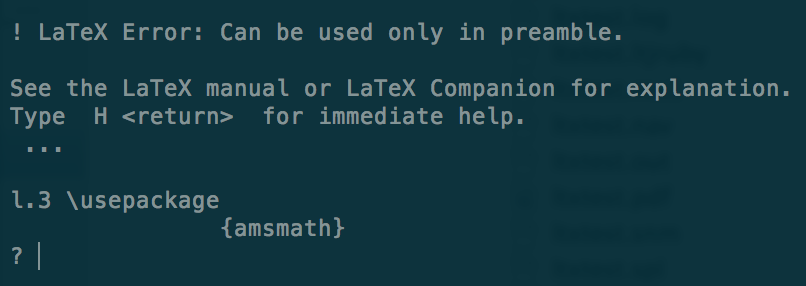
\includegraphics[width = \linewidth]{error.png}
\end{column}
\end{columns}
\begin{itemize}
  \item 叹号开始的第一行给出了错误的类型。\pause
  \item 随后的部分是 \LaTeX{} 给出的建议。\pause
  \item 字母 \texttt{l} 给出的是错误发生的位置,注意截断处。\pause
  \item 问号开始的地方正在等待用户输入。
\end{itemize}
\end{frame}

\begin{frame}{遇到报错怎么办?}
接下来,根据错误提示,检查代码,尝试修复。

若暂时无法修复,可以整理好问题提问求助。请阅读\\
\url{http://ptex.tk}
\end{frame}

\begin{frame}{有哪些值得推荐的 \LaTeX 主题网站/论坛?}
中文的有
\begin{itemize}
  \item \CTeX 论坛:\url{http://bbs.ctex.org}
  \item \ChinaTeX 论坛:\url{http://bbs.chinatex.org}
  \item \LaTeX{}studio 博客:\url{http://www.latexstudio.net}
  \item 水木论坛 \TeX{} 板块:\url{http://www.newsmth.net/nForum/\#!board/TeX}
\end{itemize}
英文的有
\begin{itemize}
  \item \TeX.SX:\url{http://tex.stackexchange.com}
  \item \LaTeX{} Community:\url{http://www.latex-community.org}
\end{itemize}
\end{frame}

\begin{frame}[fragile]{怎样方便地切换字体?}
最好的办法是使用 \XeLaTeX{} 编译。
\begin{itemize}
  \item \pkg{fontspec} 宏包用于切换西文字体
  \item \pkg{xeCJK} 宏包用于切换 CJK 字体
  \item \pkg{unicode-math} 或 \pkg{mathspec} 宏包用于选择数学字体
\end{itemize}

举一个例子。

\small
\begin{minted}{tex}
%!TEX program = xelatex
\documentclass{article}
\usepackage{xeCJK} % loads fontspec automatically
\newCJKfontfamily\cdemo{FZDHTK.ttf}
\newfontfamily\edemo{Papyrus}
\begin{document}
{\cdemo 这里是方正大黑体。}

{\edemo This is the font Papyrus.}
\end{document}
\end{minted}
\end{frame}

\begin{frame}{怎样方便地切换字体?}
\centerline{
\includegraphics[width = 0.9\linewidth]{fontdemo.png}}
\end{frame}

\begin{frame}[fragile]{怎样输出中文数字?}
最简单的办法是使用 \pkg{ctex} 宏包/文档类。

\begin{itemize}
  \item \verb|\chinese{<counter>}| 用于将计数器输出调整为中文
  \item \verb|\CTEXnumber{结果}{数字}| 用于将阿拉伯数字转换成中文数字,并将值保存在结果当中。
\end{itemize}

\begin{columns}
  \begin{column}{0.5\linewidth}
  \small
\begin{minted}{tex}
%!TEX program = xelatex
\documentclass{ctexart}
\CTEXsetup
  [number = \chinese{section}]
  {section}
\begin{document}
\setcounter{section}{123}
\section{←看这里}
\CTEXnumber{\result}{1234567}
\result
\end{document}
\end{minted}
  \end{column}
  \begin{column}{0.5\linewidth}
  \centerline{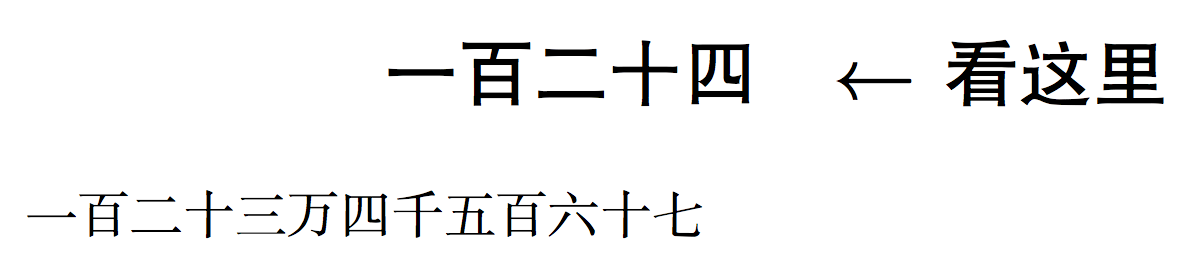
\includegraphics[width = 0.9\linewidth]{cjknumber.png}}
  \end{column}
\end{columns}
\end{frame}

\section*{关于我}

\begin{frame}{关于我}
  黄晨成,毕业于山东大学数学学院,与人合著有《GRE 基础填空 24 套精析与精练》(原稿使用 \LaTeX 排版);2010 年接触 \LaTeX,是 \pkg{xprintlen}, \pkg{sduthesis} 和 \pkg{mcmthesis} 等宏包的作者,2013 年加入 \pkg{ctex-kit},同年与邓东升一同建立 ElegantLaTeX,发布 \pkg{ElegantBook} 等模板。

  主页:\url{http://liam0205.me}

  电邮:\href{mailto:liamhuang0205@gmail.com}{liamhuang0205@gmail.com}
\end{frame}

\begin{frame}
  \sectionframe{诚征女友}
\begin{columns}
  \begin{column}{0.5\linewidth}
  \centering
  \rotatebox{-90}{\makebox[10em][s]{~~\rotatebox{90}{机}~\rotatebox{90}{智}~\rotatebox{90}{幽}~\rotatebox{90}{默}~\rotatebox{90}{才}~\rotatebox{90}{情}~\rotatebox{90}{高}}}
  \end{column}
  \begin{column}{0.5\linewidth}
  \centering
  \rotatebox{-90}{\makebox[10em][s]{~~\rotatebox{90}{温}~\rotatebox{90}{柔}~\rotatebox{90}{体}~\rotatebox{90}{贴}~\rotatebox{90}{身}~\rotatebox{90}{材}~\rotatebox{90}{好}}}
  \end{column}
\end{columns}
\end{frame}

\end{document}
